\graphicspath{{figures/figures_intro/}}


\section{The Standard Cosmological Model and Large-Scale Structure}

The universe is impressively well-described by a relatively simple cosmological model.
This model, known as $\Lambda$CDM, posits that the vast majority of the matter in the universe is composed of cold dark matter (CDM), which interacts with normal matter via (primarily, if not only) gravity, and that the accelerating expansion of the universe caused by dark energy can be described by a cosmological constant $\Lambda$.
$\Lambda$CDM can be parameterized by just a handful of quantities, including the matter energy density $\om$, the baryon energy density $\Omega_{b}$, the amplitude of matter fluctuations on a scale of 8 $\hMpc$ $\sig$, the dimensionless Hubble constant $h$, the spectral index of the primordial power spectrum $n_{s}$, and the number of relativistic species $N_{\mathrm{eff}}$. 

In the standard picture of cosmology, the very early universe underwent a period of \emph{inflation} which expanded its scale by a factor of $\simo e^{60}$.
This stretched quantum fluctuations to macroscopic scales, with small matter overdensities growing under gravity to form the large-scale structure (LSS) of the universe we observe today.
This overdensity field $\delta(\rvec)$ as a function of comoving scale $\rvec$ can be defined as
\begin{equation}
    \delta(\rvec) = \frac{\rho(\rvec) - \bar{\rho}}{\bar{\rho}}
\end{equation}
where $\rho(\rvec)$ is the density field and $\bar{\rho}$ is the mean density.

The density field can be quantified with $N$-point statistics (e.g. \citealt{peebles_large-scale_1980}).
The two-point function $\xi(r)$ is extremely informative and is the key statistic for large-scale structures studies, defined as
\begin{equation}
    \label{eq:xi}
    \xi(\rvec) = \langle \delta(\x) \delta(\x + \rvec) \rangle ~,
\end{equation}
the expectation value of the correlations between the overdensity field at comoving positions $\x$ and $\x+\rvec$.
The two-point function is assumed to be spherically symmetric so is often given as $\xi(r)$.
Two-point clustering can also be described in Fourier space by the power spectrum $P(k)$, the Fourier transform of $\xi(r)$; in principle these carry equivalent information, but in practice they have different limitations and subtleties.
In the rest of this dissertation we focus on real-space analyses.

%There is substantial evidence for the $\Lambda$CDM model.
%While $\Lambda$CDM is consistent with many of our observations, there remain open questions and inconsistencies that hint at a more complex model or a deeper underlying explanation.

The large-scale distribution of matter in the universe is a key cosmological observable.
As most of the matter is in the form of dark matter (DM), which has remained undetectable by direct methods, to make measurements from LSS we must infer the distribution of DM from luminous tracers.
Baryonic matter collects in dense regions of DM and, over cosmic time, evolves into the galaxies we observe today.

However, galaxies are not direct tracers of the underlying matter field; rather, they are \emph{biased} tracers with a different spatial distribution than the dark matter \citep{kaiser_spatial_1984}.
While the relationship between the galaxy overdensity field $\delta_g$ and DM overdensity field $\delta$ could be some general function, it is well-described by a linear bias parameter $b_g$,
\begin{equation}
    \delta_g = b_g \delta ~.
\end{equation}
Relating this to the correlation function with \eqref{eq:xi}, we obtain
\begin{equation}
    \xi_g^2 = b_g \xi^2
\end{equation}
where $\xi_g$ is the correlation function of galaxies.
Different types of galaxies exhibit somewhat different clustering properties and thus values for $b_g$, but these are typically in the range $1<b_g<2$.

To use the distribution of galaxies to infer the underlying large-scale structure---as well as to understand galaxy formation---we must model in more detail the connection between galaxies and dark matter.
This is discussed in the next section.


\section{The Connection between Dark Matter and Galaxies}
\label{sec:galhalo}


The standard cosmological model describes a picture in which the initially small overdensities eventually collapse and form gravitationally bound regions of dark matter known as \emph{halos} (e.g. \citealt{bryan_statistical_1998}) which continue to grow and merge with each other.
Galaxies evolve within halos, growing by forming stars and accreting matter from mergers; galactic processes affect the dark matter environment through \emph{feedback}.
The properties of baryons and the complicated physics of galaxy formation impact the relationship between dark matter and galaxies.

\begin{figure*}
    \centering
    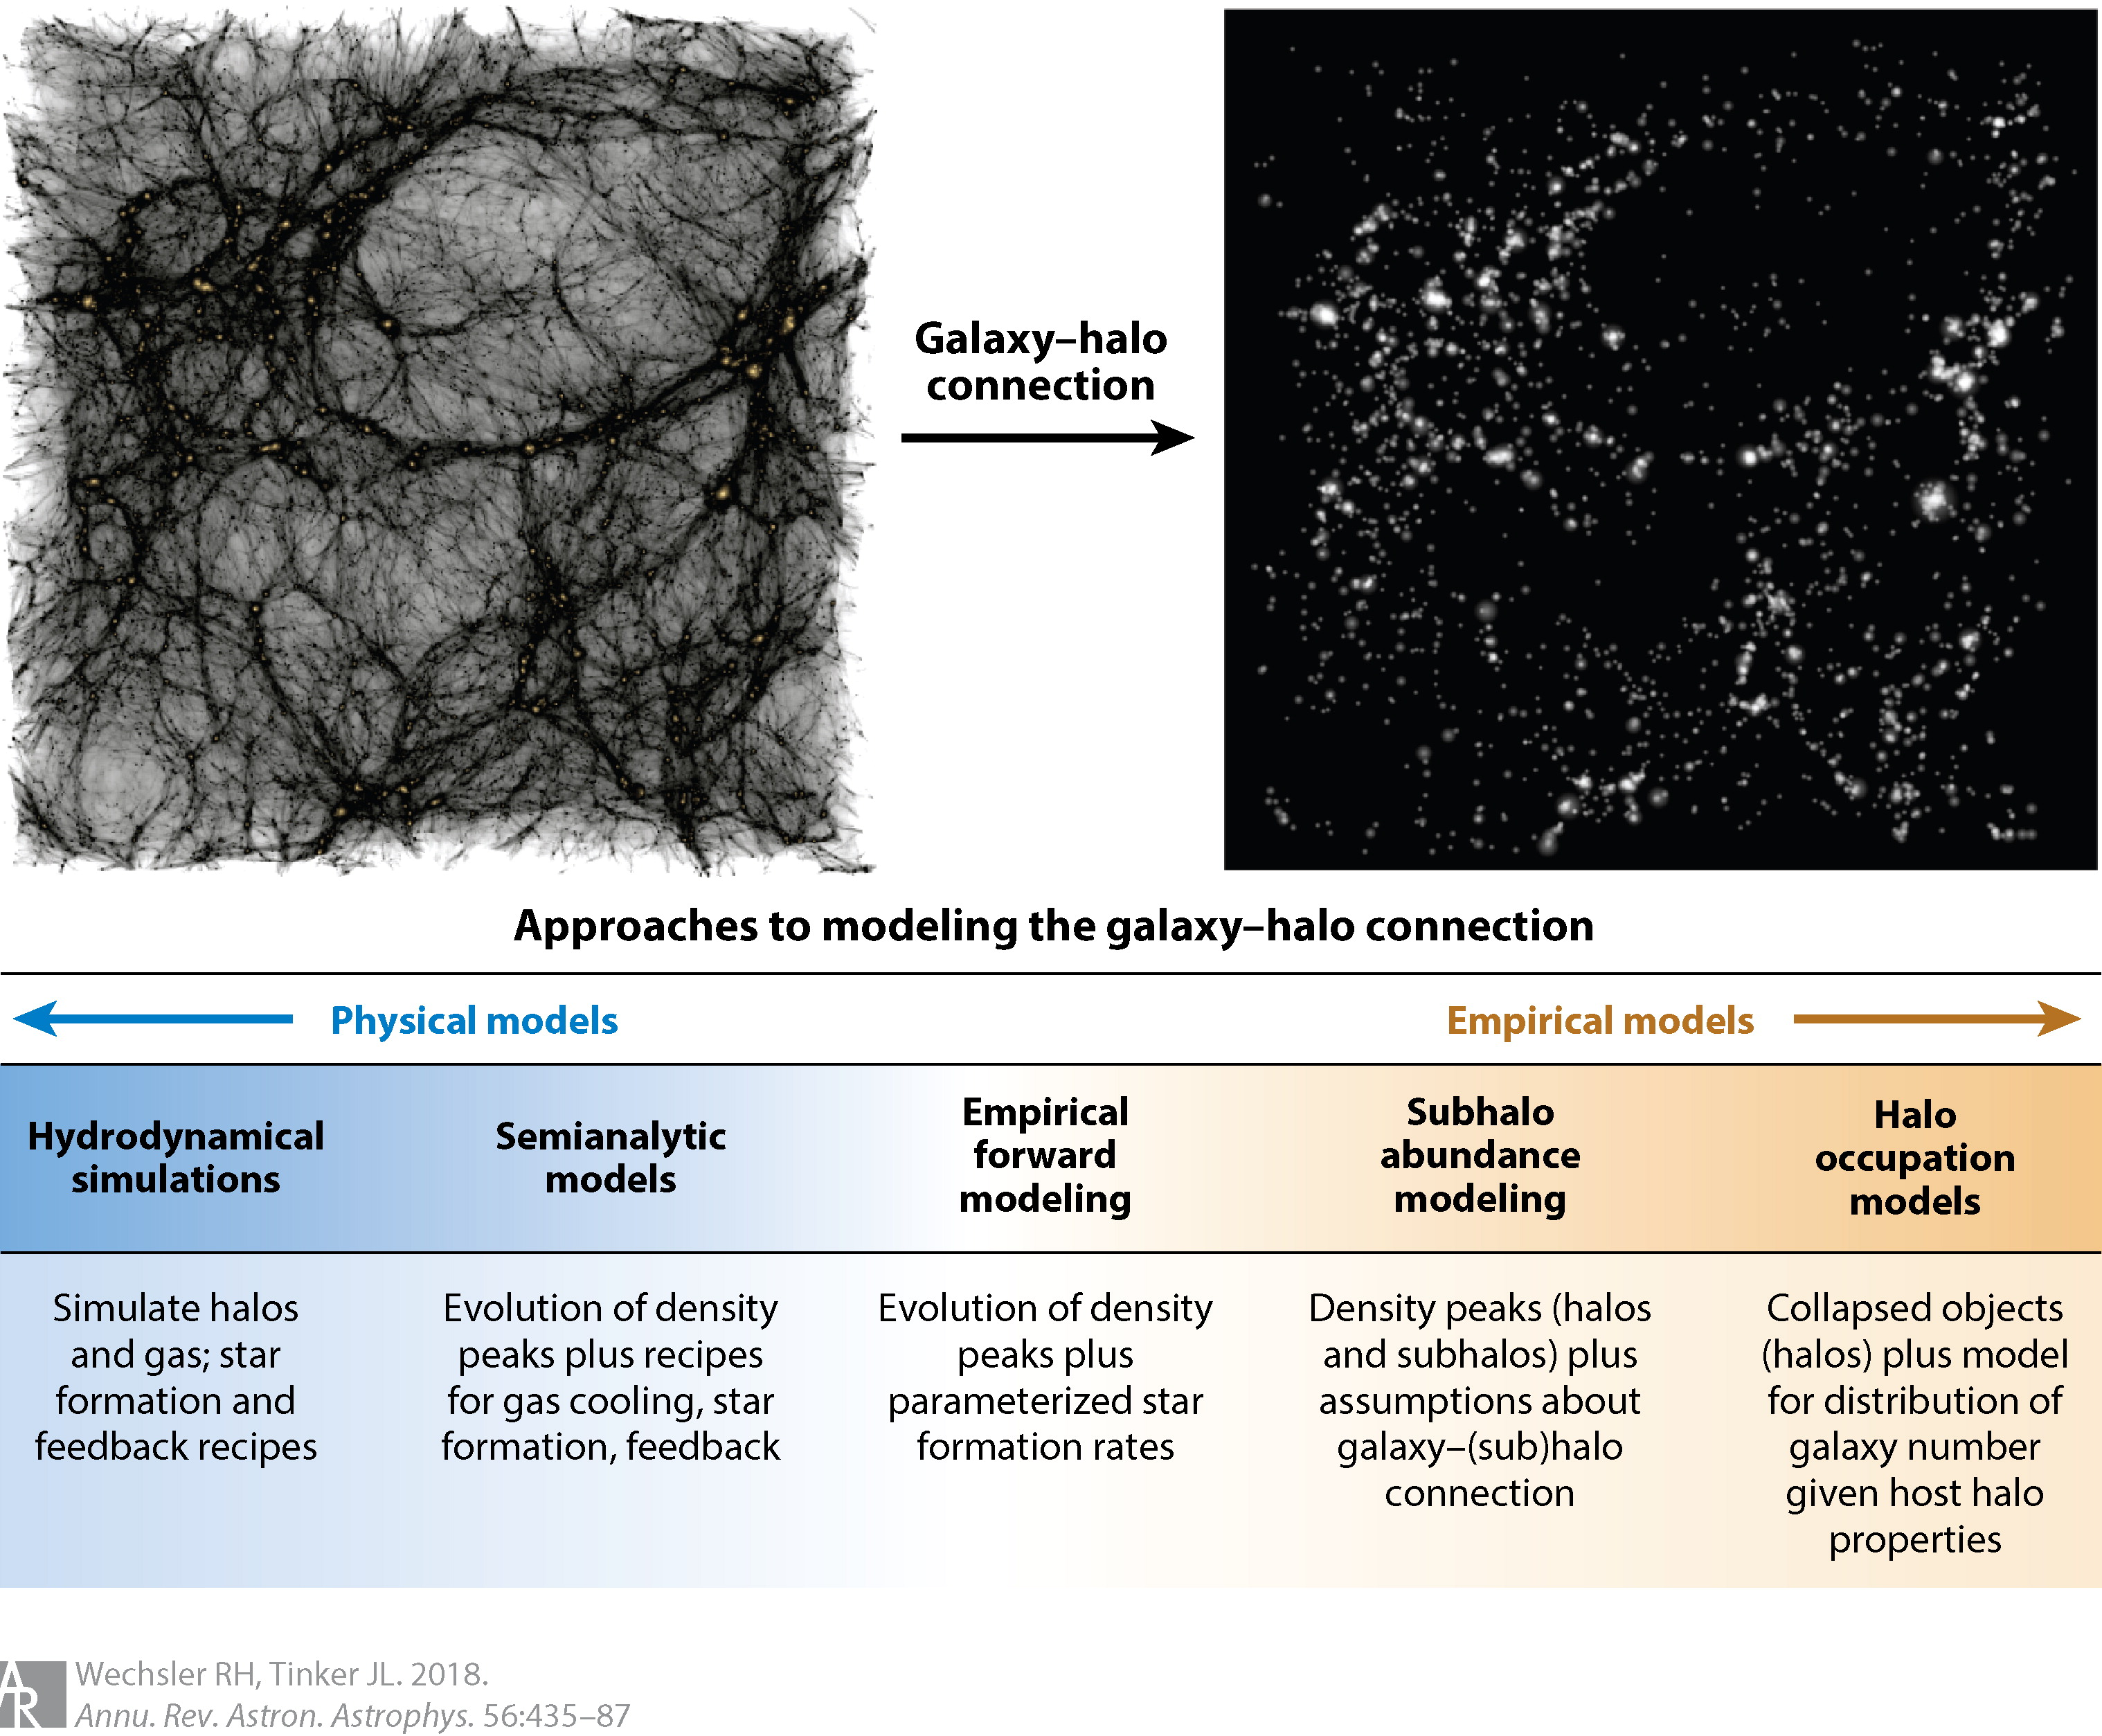
\includegraphics[width=0.9\textwidth]{galhalo.jpg}
    \caption{A visualization of the galaxy--halo connection and a range of modeling approaches. The top panel shows the dark matter distribution in a slice of a cosmological simulation, and the corresponding galaxy population modeled using abundance matching. The bottom panel outlines approaches ranging from physical models to empirical models for modeling the relationship between dark matter and galaxies. \emph{Figure 1 of \cite{wechsler_connection_2018}.}}
    \label{fig:galhalo}
\end{figure*}

This relationship is visualized in Figure~\ref{fig:galhalo}, showing the DM distribution of a cosmological simulation paired with its galaxy population using an empirically calibrated model.
The figure also outlines a range of models from the literature for describing this connection, from empirical to physical models.
A comprehensive review can be found in \cite{WechslerTinker2018}.
Here I describe the models at each end of this range, as these are the ones utilized in this dissertation, but each model on this spectrum has important uses.

A description of the galaxy--halo connection that has proven broadly successful is \emph{halo occupation distribution} (HOD) modeling (e.g. \citealt{peacock_halo_2000,Seljak2000,BerlindWeinberg2002}). 
The HOD model posits the conditional distribution of the number of galaxies $N$ occupying a halo, typically conditioned on halo mass $M$: $P(N|M)$.
This model has only a handful of parameters while remaining flexible enough to fit observed galaxy samples well (e.g. \citealt{Zheng2005,reddick_connection_2013}).
However, this ``vanilla'' HOD is not sufficient.
Analyses have shown that the clustering of halos depends on halo properties beyond mass, including formation time and concentration, an effect is known as \emph{halo assembly bias} \citep{wechsler_concentrations_2002, Wechsler2006,mao_beyond_2018}.
This may propagate to the clustering of galaxies, dubbed \emph{galaxy assembly bias}, and must be taken into account in HOD modeling (e.g. \citealt{Tinker2008,hearin_introducing_2016}).
An HOD model with environment-dependent assembly bias is used in the cosmological inference approach presented in Chapter~\ref{chp:aemulus}, in which the parameters of the HOD are marginalized over.

On the other end of the spectrum, cosmological hydrodynamic simulations aim to model the relationship between dark matter and galaxies based on deeper physical underpinnings (e.g. \citealt{springel_gadget_2001, genel_introducing_2014,dave_simba_2019}).
These co-evolve dark matter and baryons under gravity and hydrodynamics in cosmological volumes (typically $\simo 25 < L < \simo 300$); given the large dynamic range of relevant physical scales, galaxies cannot be fully simulated but instead rely on ``subgrid models'' that are empirically calibrated.
With these models, simulations can include stellar winds, feedback from active galactic nuclei, gas cooling, and supernovae feedback, among other processes; a detailed review can be found in \cite{somerville_physical_2015}.
These galactic processes can both impact the dark matter environment as well as display degeneracies with cosmological effects (see e.g. \citealt{villaescusa-navarro_camels_2021}), making robust modeling of them crucial to understanding galaxy clustering.
In their current state, hydrodynamic simulations make too many assumptions to be applicable to cosmological inference, but they are useful in their own right to explore{\emdash}given the input assumptions{\emdash}how dark matter properties are related to galaxy properties.

Despite significant progress, the galaxy--halo connection remains a large area of uncertainty, largely due to poorly constrained galaxy formation physics.
As this relationship is a critical ingredient of cosmological inference, efforts to understand and model it are paramount.
One such effort is explored in Chapter~\ref{chp:eqcosmo}, using the IllustrisTNG cosmological hydrodynamic simulation \citep{springel_first_2018,nelson_first_2018,pillepich_first_2018,naiman_first_2018,marinacci_first_2018}. 


\section{Redshift Surveys}

Over past several decades, we have built up immense 3-dimensional maps of the universe through observations of millions of galaxies.
These involve initial targeting using wide-field imaging, followed by spectroscopic observations to measure galaxy \emph{redshifts}.
The redshifts, measured by the shift of spectral lines from their rest-frame wavelength, indicate the velocity at which a galaxy is moving away from us and thus (assuming the velocity is dominated by the Hubble flow) its distance.
Early photographic observations of galaxies and  analyses of their angular distribution detected non-uniformity below a certain scale \citep{shapley_survey_1932,hubble_distribution_1934,seldner_new_1977,peebles_galaxy_2001}.
These results were extended to three dimensions by early redshift surveys, including \cite{gregory_comaa1367_1978} (238 galaxies around the Coma cluster), the KOS survey (\citealt{kirshner_million_1981}, 133 galaxies), and the CfA survey (\citealt{davis_survey_1982}, $\simo$2400 galaxies).
These confirmed the clustered distribution of galaxies, which can be identified visually even from these small samples. 
Figure~\ref{fig:cfa_survey} shows a sample of galaxies from the CfA survey, about which the authors remark that the regions ``exhibit clustering in frothy, almost filamentary, patterns of connectedness surrounding empty holes on the sky.''

\begin{figure*}
    \centering
    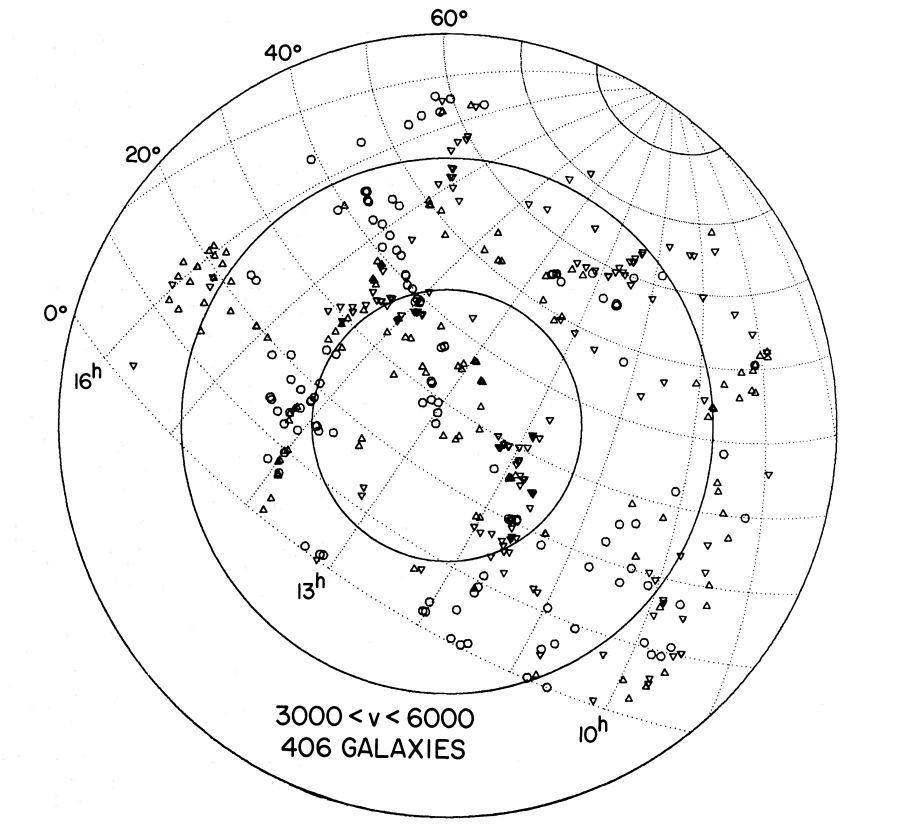
\includegraphics[width=0.6\textwidth]{cfa_survey}
    \caption{A sample of galaxies from the CfA redshift survey. Galaxies in the North Galactic Cap with $M<-18.5$ and velocity $3000<v<6000$ km s$\inv$ are shown in an equal-area sky projection. Filamentary structures, clusters, and voids can be seen visually. \emph{Figure 2b. of \cite{davis_survey_1982}.}}
    \label{fig:cfa_survey}
\end{figure*}

Modern redshift surveys have now observed orders of magnitude more galaxies and used their distributions to obtain some of the most stringent constraints on cosmological parameters.
The 2dF Galaxy Redshift survey \citep{Colless2001} observed $\simo$250,000, add the Sloan Digital Sky Survey (SDSS, \citealt{York2000}) observed nearly one million galaxy redshifts.
Galaxy power spectrum analyses of these surveys achieved measurements of the matter density ${\om}$ with a precision of $\simo$10\% \citep{cole_2df_2005, tegmark_cosmological_2006}.
Combining the results of baryon acoustic oscillations and redshift-space distortion analyses, SDSS has measured the parameter $\sig$ to $\simo$3.5\%; a joint analysis with other cosmological measurements, including the cosmic microwave background, supernovae, and weak lensing, results in $\simo$1\% precision.

\begin{figure}
    \centering
    \includegraphics[width=0.52\textwidth]{desi_survey.jpg}
    \caption{A sample of galaxies from the DESI survey, around 40 years after the CfA survey of Figure~\ref{fig:desi_survey}. Around 400,000 galaxies are shown, out to $z \sim 0.9$ (3 $\hGpc$). DESI will observe nearly an order of magnitude more redshifts than this over the course of the survey. \emph{D. Schlegel/Berkeley Lab using data from DESI. Acknowledgment: M. Zamani (NSF's NOIRLab).}}
    \label{fig:desi_survey}
\end{figure}

Efforts are ongoing to map even more galaxies to increase the constraining power of large-scale structure.
The Dark Energy Spectroscopic Instrument (DESI, \citealt{Aghamousa2016}) has already cataloged nearly ten million redshifts and will observe multiple times that over the rest of the mission.
A slice through a sample of the galaxies DESI has already observed is shown in Figure~\ref{fig:desi_survey}; the filamentary structure hinted at in the CfA survey is now clear across the sky, and filaments are even cataloged and studied as objects in their own right (e.g. \citealt{tempel_detecting_2014}).
Future surveys are planned to measure yet more galaxy redshifts, including the Subaru Prime Focus Spectrograph \citep{takada_extragalactic_2014}, Euclid \citep{Laureijs2011}, and the Nancy Grace Roman Space Telescope \citep{Green2012}.
This galaxy clustering data is so high-precision that the bottleneck for cosmological constraints will lie largely in our modeling and analysis methodologies; one such improved approach, targeted at SDSS or DESI data, is presented in Chapter~\ref{chp:aemulus}.

While galaxies are the dominant tracer observed for large-scale structure surveys given their multitude, other types of sources also provide valuable information.
Quasars, which are extremely luminous emission from active galactic nuclei{\emdash}accreting supermassive black holes{\emdash}at the centers of galaxies, are even more highly biased tracers of matter than galaxies, with $b \sim 2.5$ at $z \sim 1.5$ \citep{laurent_clustering_2017-3}.
Redshift surveys of quasars are the largest-volume maps of the universe we have, as we can observe quasars at immense distances thanks to their high luminosity.
Millions of quasars have been observed, with hundreds of thousands having spectroscopic redshifts, and more are being cataloged by current missions.
One such mission, \emph{Gaia}, and the opportunities it presents for large-scale structure science with quasars is discussed further in Chapter~\ref{chp:quaia}.



\section{Cosmological Inference from Galaxy Clustering}

\begin{figure*}
    \centering
    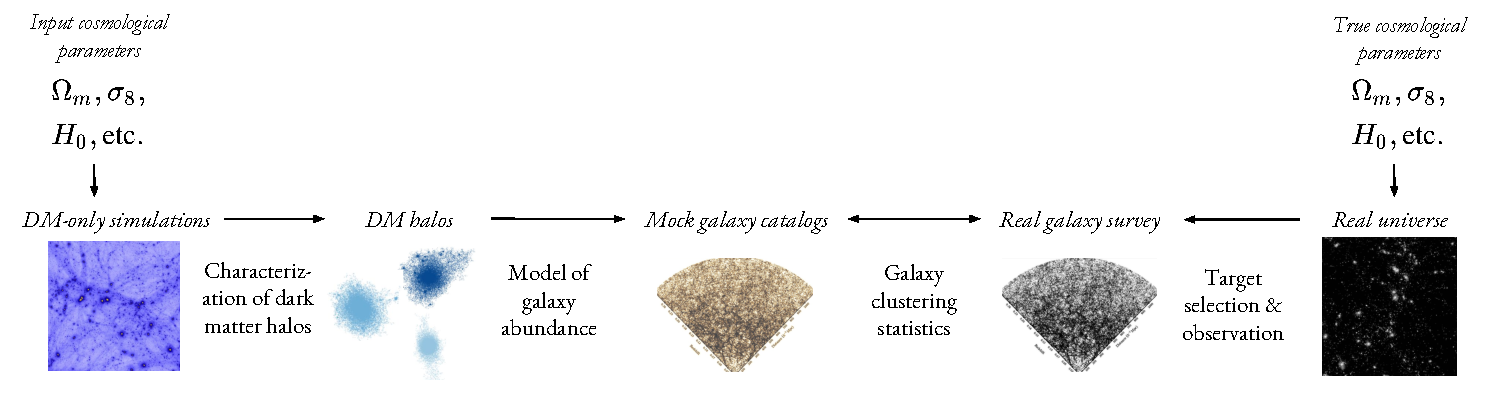
\includegraphics[width=\textwidth]{cosmo_inference.pdf}
    \caption{A schematic of a simulation-based cosmological inference pipeline. From the simulation side, dark matter only cosmological simulations are run with various input cosmological parameters; dark matter halos are identified and populated with galaxies to produce a mock galaxy catalog. On the observation side, the distribution of galaxies depends on the cosmological quantities, and these are cataloged in redshift surveys. Clustering statistics can then be used to compare real and mock surveys and estimate best-fit model parameters.}
    \label{fig:cosmo_inf}
\end{figure*}

The distribution of galaxies is extremely high-dimensional and complex, such that the actual positions of individual galaxies are impossible to model directly.
Luckily, these are largely irrelevant to the underlying cosmology that we care about; rather, the cosmological model makes strong predictions about the \emph{statistical} properties of the large-scale structure.
By computing the statistics of the galaxy distribution, we can compare our observations to models and infer the cosmological and astrophysical model parameters, as well as learn where our models are insufficient to describe the data.

Standard cosmological inference from galaxy clustering relies on low-order statistics of the galaxy distribution.
The most important statistic is the \emph{two-point correlation function} (\cf), denoted $\xi(r)$, which is defined as the excess probability $\delta P$ of finding a galaxy in a volume element $\delta V$ a given separation $r$ apart from another galaxy compared to a random distribution:
\begin{equation}
    \delta P = n[1+\xi(r)]\delta V ~,
\end{equation}
where $n$ is the mean galaxy number density.
Below scales of $r \sim 10 \hMpc$, the \cf roughly follows a power law, $\xi(r) \sim (r/r_0)^{-\gamma}$, where $r_0$ is a characteristic scale (found to be $r_0 \sim 5 \hMpc$) and $\gamma$ is the power law index, measured to be $\gamma \sim 1.8$.
The \cf can be estimated from galaxy samples with estimators that take into account the finite, irregular window function of the survey, using estimators such as that proposed by \cite{DavisPeebles1983} or \cite{LandySzalay1993}.
In Chapter~\ref{chp:cfe} these are discussed in much more detail, and a generalized estimator for the \cf is presented.

There is also significant cosmological information beyond the two-point function.
A slew of statistics aim to capture this information, including the three-point statistic (the bispectrum, in Fourier space), void statistics (e.g. \citealt{sheth_hierarchy_2004}), and environment-based statistics (e.g. \citealt{Sheth2004,tinker_void_2007}).
These can be more difficult to measure and model than the \cf, but are critical for breaking certain degeneracies (e.g. \cite{WhitePadmanabhan2009}).
Recently full field-level inference has shown promise, such as EFTofLSS \citep{baumann_cosmological_2012}.

The measured statistics can then be compared to a model prediction to estimate the model parameters that most closely describe the data.
Some of these statistics can be modeled analytically, using perturbation theory; this is the standard for many major analyses (e.g. \citealt{tegmark_cosmological_2006}) 
However, this is only possible at large scales (and for other statistics not at all), where the evolution of structure is largely linear and galaxy physics has a weaker effect.
There is significant cosmological information at small scales; accessing it requires the use of cosmological simulations.
While these are far too expensive to run at each point in parameter space, other robust inference approaches have been developed. 
These include simulation-based inference (SBI, e.g. \citealt{hahn_rm_2022}), and emulation of simulations (e.g. \citealt{Heitmann2009, Lawrence2017, Angulo2021}); the latter approach is the basis for Chapter~\ref{chp:aemulus}.
In these cases, $N$-body simulations are run at many points in cosmological parameter space, and populated with galaxies with a galaxy--halo connection model such as those discussed in \S\ref{sec:galhalo}.
These astrophysical model parameters can then marginalized over to obtain constraints on cosmological parameters.
A schematic of a possible pipeline for cosmological inference using simulations is shown in Figure~\ref{fig:cosmo_inf}.

There are numerous other elements to robust cosmological inference.
A key such element is the construction of a covariance matrix, as the data vector components are often highly correlated; computation or estimation of the covariance matrix is required for likelihood-based inference approaches (while likelihood-free inference approaches such as SBI avoid this issue).
The approach that has now become standard for large-scale structure analyses is to estimate the covariance many \emph{mock catalogs} of the expected galaxy distribution, requiring on the order of 1000 mocks to get a reasonable estimate \citep{Anderson2012,Kitaura2016,Beutler2017}.
Given the cost of simulations, covariance matrix estimation is one of the limiting steps of cosmological inference.
Another critical element is systematics mitigation: observational and instrumental effects project onto the galaxy distribution and can mimic or obscure cosmological signals.
These and other issues and approaches for cosmological inference are discussed in further detail in the following Chapters.


\section{Chapter Notes}

In this thesis, I present new tools for studying large-scale structure and galaxy formation from multiple angles.
These tools range from statistical and machine learning methods to simulation-based approaches and observational data catalogs.

In Chapter~\ref{chp:aemulus}, I present an approach for cosmological inference using probabilistic machine learning and N-body simulations, and demonstrate the importance of environment-dependent clustering statistics.
In Chapter~\ref{chp:cfe}, I develop a new statistic for galaxy clustering that obviates issues of traditional, binned clustering statistics.
I explore a new approach to characterizing the dark matter distribution in cosmological simulations using symmetry-preserving quantities in Chapter~\ref{chp:eqcosmo}, relevant to understanding the galaxy--halo connection.
Chapter~\ref{chp:quaia} presents the largest-volume spectroscopic quasar catalog ever constructed, based on \emph{Gaia} and unWISE, which is an unprecedented sample for large-scale structure analyses.
Finally, in Chapter~\ref{chp:anomalies} I look at using deep learning to identify anomalous galaxy images with the goal of widening the discovery possibilities of galaxy surveys.

Chapters~\ref{chp:cfe} and \ref{chp:anomalies} have been refereed and published in the astronomical literature (\emph{The Astrophysical Journal} and \emph{Monthly Notices of the Royal Astronomical Society}, respectively).
Chapter~\ref{chp:aemulus} has been submitted to \emph{The Astrophysical Journal} and is under review.
Chapters~\ref{chp:eqcosmo} and \ref{chp:quaia} are in the final draft stage and will be submitted to journals soon.
The code associated with all of these chapters is publicly available online.\footnote{\url{https://github.com/kstoreyf}}

While the analyses in each Chapter were conducted in collaboration with my co-authors and the support of many others, the majority of the work and the (near-)entirety of the writing in this dissertation is mine. 
I describe the contributions of myself and my coauthors to each Chapter here:
\begin{enumerate}[leftmargin=4\parindent]
    \item[Chapter~\ref{chp:aemulus}:] I developed the idea for this project with Jeremy Tinker and the rest of the \aemulus collaboration. I led the development of this project in conjunction with Jeremy Tinker, with input from Zhongxu Zhai, Joseph DeRose, Risa H. Wechsler, and Arka Banerjee. I implemented all of the code, which used Zhongxu Zhai's code as a starting point and simulations led by Joseph DeRose. I wrote the paper text and received feedback from the rest of the collaboration.
    \item[Chapter~\ref{chp:cfe}:] I developed the idea for this project with David W. Hogg. I implemented the code and worked out the mathematical proof. I wrote the paper with input from David W. Hogg.
    \item[Chapter~\ref{chp:eqcosmo}:] I conceived the idea for this project, and developed it in collaboration with David W. Hogg, Shy Genel, and Soledad Villar. I implemented it with additional feedback from Soichiro Hattori, Austen Gabrielpillai, and Yongseok Jo. I wrote the chapter text, with feedback from these collaborators.
    \item[Chapter~\ref{chp:quaia}:] I developed the idea for this project in collaboration with David W. Hogg and Hans-Walter Rix. I implemented it with additional feedback from Anna-Christina Eilers and Giulio Fabbian. I wrote the text of the chapter with input from these collaborators.
    \item[Chapter~\ref{chp:anomalies}:] The idea for this project was conceived at the Kavli Summer Program in Astrophysics in 2019, in collaboration with Marc Huertas-Company and Alexie Leauthaud. I led project development and implementation, with feedback from Nesar Ramachandra, Francois Lanusse, and J. Xavier Prochaska. Yifei Luo took observations and reduced the data, Song Huang contributed data support, and J. Xavier Prochaska contributed analysis support. I wrote the text of the paper with input from these collaborators.
\end{enumerate}


